%
%  chapter2.tex — Enquadramento e Estado da Arte
%
\chapter{Enquadramento e Estado da Arte}
\label{cha:enquadramento}

\section{Cidades Inteligentes e Sustentabilidade}
\label{sec:smart_cities}

O conceito de cidade inteligente (\textit{smart city}) refere-se a um ecossistema urbano que integra tecnologias de informação e comunicação com o objetivo de melhorar a qualidade de vida dos seus habitantes, otimizar a gestão de recursos e promover a participação cívica~\cite{neirotti2014current}. A transição para este modelo exige não apenas investimento em infraestrutura, mas também o desenvolvimento de literacia digital e ambiental por parte dos cidadãos.

Os ODS~4, 11 e~13 das Nações Unidas estabelecem metas concretas neste domínio: o primeiro apela à criação de cidades e comunidades sustentáveis e inclusivas; o segundo à adoção de medidas urgentes para combater as alterações climáticas. Ambos reconhecem o papel central da educação e da sensibilização cidadã como instrumentos de mudança~\cite{un2015sdg}.

A Aliança U!REKA (\textit{University Research and Knowledge Alliance}) posiciona-se neste contexto como catalisadora de soluções inovadoras que articulem investigação académica, tecnologia e necessidades das comunidades urbanas, promovendo a transição inteligente e sustentável das cidades europeias~\cite{ureka2024}.

\section{Aprendizagem Adaptativa}
\label{sec:adaptive_learning}

A aprendizagem adaptativa (\textit{adaptive learning}) caracteriza-se pela capacidade de um sistema formativo ajustar dinamicamente o conteúdo, o ritmo e a sequência de aprendizagem com base no desempenho e nas dificuldades individuais de cada aprendente~\cite{vanlehn2011relative}. Esta abordagem tem demonstrado resultados superiores às metodologias de ensino uniformizadas, nomeadamente em contextos de aprendizagem informal e \textit{e-learning}.

Os sistemas de tutoria inteligente (\textit{Intelligent Tutoring Systems} --- ITS) constituem o paradigma clássico desta abordagem, modelando o conhecimento do aluno e intervindo proativamente quando são detetadas lacunas~\cite{bloom1984sigma}. Com o advento dos modelos de linguagem de grande dimensão (\textit{Large Language Models} --- LLMs), a geração automática de conteúdo pedagógico personalizado tornou-se acessível a plataformas de menor escala~\cite{kasneci2023chatgpt}.

\section{Gamificação na Educação}
\label{sec:gamification}

A gamificação consiste na aplicação de elementos e mecânicas de jogo em contextos não lúdicos, com o objetivo de aumentar o \textit{engagement}, a motivação e a retenção de comportamentos~\cite{deterding2011game}. Em contextos educativos, os elementos mais frequentemente utilizados incluem pontos, \textit{badges}, tabelas de classificação (\textit{leaderboards}), desafios progressivos e sistemas de recompensa~\cite{hamari2014does}.

Estudos recentes demonstram que a gamificação, quando bem integrada na estrutura pedagógica, pode aumentar significativamente a motivação intrínseca dos aprendentes e reduzir as taxas de abandono em plataformas de \textit{e-learning}~\cite{hamari2014does}. Contudo, a eficácia desta abordagem depende criticamente do alinhamento entre as mecânicas de jogo e os objetivos de aprendizagem.

\section{Microcompetências}
\label{sec:microcompetencias}

O conceito de microcompetência (\textit{micro-credential}) refere-se a uma unidade mínima de aprendizagem verificável, com um escopo temático bem delimitado e associada a um processo de validação formal~\cite{eur2022micro}. As microcompetências permitem modularizar o percurso formativo, tornando-o mais flexível, acessível e adaptado às necessidades de cada indivíduo.

A Comissão Europeia tem promovido ativamente a adoção de microcompetências no espaço europeu de educação, reconhecendo o seu potencial para responder às necessidades de requalificação (\textit{upskilling} e \textit{reskilling}) num mercado de trabalho em rápida transformação~\cite{eur2022micro}. No contexto do \textit{Play4Change}, as microcompetências constituem a unidade fundamental de progressão do aprendente, reconhecida através da atribuição de \textit{badges}.

\section{Estado da Arte}
\label{sec:estado_arte}

Nesta secção apresenta-se uma análise das principais plataformas de aprendizagem existentes, avaliando a sua adequação ao contexto do presente projeto segundo os três requisitos identificados na Secção~\ref{sec:problema}: mecanismos de \textit{engagement}, personalização adaptativa e reconhecimento formal de competências.

\textbf{Duolingo}~\cite{duolingo2024} constitui um caso de referência na gamificação da aprendizagem linguística, com mecanismos de \textit{streaks}, \textit{XP} e \textit{leagues} que promovem a regularidade e o \textit{engagement}. Contudo, o modelo é essencialmente estático no que respeita à adaptação de conteúdo e não aborda o domínio das cidades inteligentes ou da sustentabilidade.

\textbf{Khan Academy}~\cite{khanacademy2024} oferece um vasto repositório de conteúdo educativo de acesso livre, com alguns mecanismos de personalização baseados no desempenho. No entanto, a plataforma não dispõe de geração automática de conteúdo por IA nem de mecanismos de deteção de dificuldades em tempo real.

\textbf{Coursera} e \textbf{edX}~\cite{coursera2024,edx2024} são plataformas de \textit{MOOC} (\textit{Massive Open Online Courses}) com certificação reconhecida, mas orientadas para percursos formativos longos e estruturados, sem gamificação significativa nem adaptação em tempo real ao aprendente.

\textbf{Kahoot!}~\cite{kahoot2024} explora a dimensão lúdica da aprendizagem através de \textit{quizzes} competitivos, mas não dispõe de mecanismos de adaptação individual nem de reconhecimento formal de competências.

\subsection{Análise Comparativa}
\label{ssec:comparativa}

A Tabela~\ref{tab:comparativa} sintetiza a análise comparativa das plataformas identificadas face às características-chave do \textit{Play4Change}.

\begin{table}[ht]
  \caption{Análise comparativa de plataformas de aprendizagem}
  \label{tab:comparativa}
  \vskip0.5em
  \centering
  \begin{tabular}{lccc}
    \toprule
    \textbf{Plataforma} & \textbf{Gamificação} & \textbf{Desafios Adaptativos} & \textbf{Microcompetências} \\
    \midrule
    Duolingo       & \checkmark & Parcial & $\times$ \\
    Khan Academy   & Parcial    & Parcial & $\times$ \\
    Coursera / edX & $\times$   & $\times$ & Parcial \\
    Kahoot!        & \checkmark & $\times$ & $\times$ \\
    \textbf{Play4Change} & \checkmark & \checkmark & \checkmark \\
    \bottomrule
  \end{tabular}
\end{table}

A análise comparativa evidencia que nenhuma das plataformas existentes combina, em simultâneo, os três pilares identificados no Capítulo~\ref{cha:introducao}: \textbf{Engagement}, \textbf{Personalização} e \textbf{Reconhecimento}, num contexto específico de literacia cívica e sustentabilidade urbana. O \textit{Play4Change} posiciona-se assim como uma solução inovadora e diferenciada no panorama atual, conforme ilustrado na Figura~\ref{fig:posicionamento}.

\begin{figure}[htbp]
  \centering
  % TODO: substituir por img/posicionamento.pdf quando disponível
  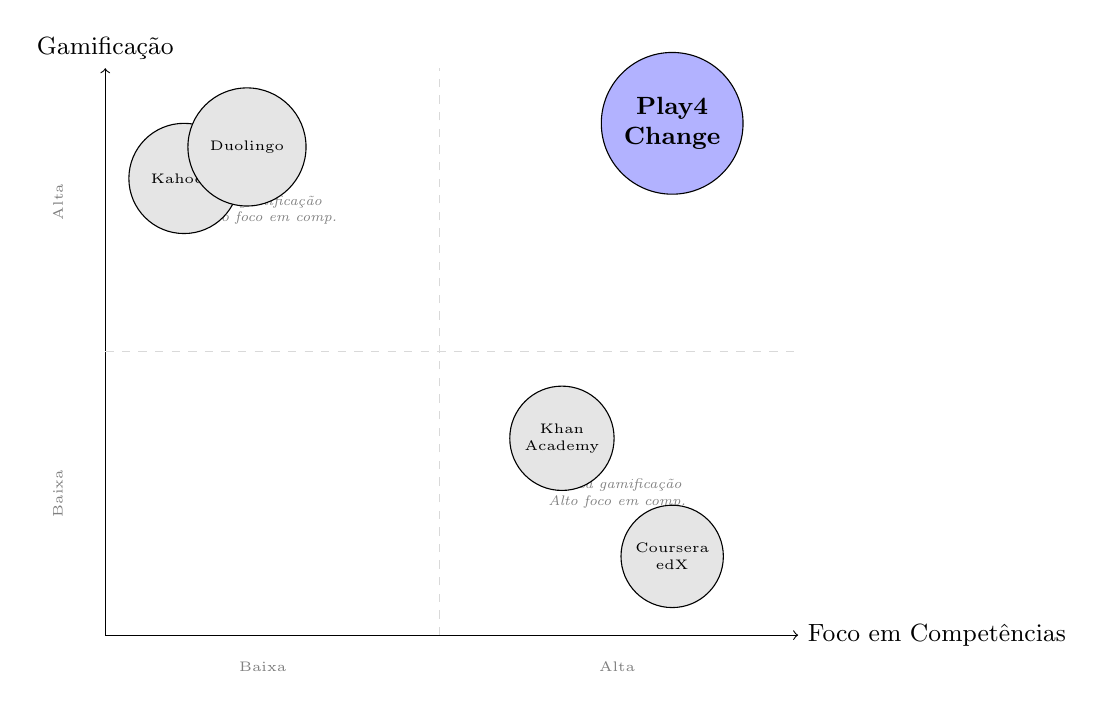
\begin{tikzpicture}[font=\small]
    % Axes
    \draw[->] (0,0) -- (8.8,0) node[right] {\small Foco em Competências};
    \draw[->] (0,0) -- (0,7.2) node[above] {\small Gamificação};
    % Axis tick labels
    \node[font=\tiny, gray] at (2.0,-0.4) {Baixa};
    \node[font=\tiny, gray] at (6.5,-0.4) {Alta};
    \node[font=\tiny, gray, rotate=90] at (-0.6, 1.8) {Baixa};
    \node[font=\tiny, gray, rotate=90] at (-0.6, 5.5) {Alta};
    % Quadrant dividers
    \draw[gray!30, dashed] (4.25,0) -- (4.25,7.2);
    \draw[gray!30, dashed] (0,3.6) -- (8.8,3.6);
    % Quadrant labels
    \node[font=\tiny\itshape, gray, align=center] at (2.0, 5.4)
      {Alta gamificação\\Baixo foco em comp.};
    \node[font=\tiny\itshape, gray, align=center] at (6.5, 1.8)
      {Baixa gamificação\\Alto foco em comp.};
    % Platform bubbles
    % Coursera/edX: gamificação=× (y~1.0), aprendizagem profunda (x~7.2)
    \node[draw, circle, fill=gray!20, minimum size=1.3cm, font=\tiny, align=center]
      at (7.2, 1.0) {Coursera\\edX};
    % Khan Academy: gamificação=Parcial (y~2.5), aprendizagem profunda (x~5.8)
    \node[draw, circle, fill=gray!20, minimum size=1.3cm, font=\tiny, align=center]
      at (5.8, 2.5) {Khan\\Academy};
    % Kahoot!: gamificação=✓ (y~5.8), aprendizagem superficial (x~1.0)
    \node[draw, circle, fill=gray!20, minimum size=1.4cm, font=\tiny, align=center]
      at (1.0, 5.8) {Kahoot!};
    % Duolingo: gamificação=✓ (y~6.2), aprendizagem superficial (x~1.8)
    \node[draw, circle, fill=gray!20, minimum size=1.5cm, font=\tiny, align=center]
      at (1.8, 6.2) {Duolingo};
    % Play4Change: gamificação=✓ (y~6.5), microcompetências=✓ (x~7.2) — unique top-right
    \node[draw, circle, fill=blue!30, minimum size=1.8cm, align=center,
          font=\small\bfseries]
      at (7.2, 6.5) {Play4\\Change};
  \end{tikzpicture}
  \caption{Mapa de posicionamento das plataformas (Gamificação vs.\ Foco em Competências)}
  \label{fig:posicionamento}
\end{figure}

É neste contexto que o Capítulo~\ref{cha:solucao} apresenta a solução proposta, descrevendo a arquitetura e os componentes do \textit{Play4Change} concebidos para colmatar a lacuna identificada.
